% % This is cool: https://bayes.wustl.edu/etj/articles/leapz.pdf
\documentclass[aspectratio=169,dvipsnames,18pt]{beamer}

\input{talkPreambleNoBeamer.tex}
\usepackage{physics}
\usepackage{fancyvrb}
\usepackage{annotate-equations}

\mode<presentation>
{
  \usetheme{Malmoe}
  \usefonttheme{serif}

  \setbeamertemplate{headline}{}
  \setbeamertemplate{footline}{}
  \setbeamercovered{transparent}
}

\AtBeginSection[]
{
  \begin{frame}<beamer>
    \frametitle{Outline}
    \tableofcontents[currentsection,hideothersubsections]
  \end{frame}
}

\AtBeginSubsection[]
{
  \begin{frame}<beamer>
    \frametitle{Outline}
    \tableofcontents[sectionstyle=show/hide,subsectionstyle=show/shaded/hide]
  \end{frame}
}

\setbeamerfont{title}{size=\normalsize}
\setbeamerfont{author}{size=\footnotesize,series=\bfseries}
\setbeamerfont{title page}{size=\scriptsize}

\setbeamercovered{invisible}

% Bibliography
%   http://tex.stackexchange.com/questions/12806/guidelines-for-customizing-biblatex-styles
\usepackage[sorting=none, backend=biber, style=authoryear, maxcitenames=4, maxbibnames=20]{biblatex}
\addbibresource{presentations.bib}
\renewcommand*{\bibfont}{\tiny}

\title[Bayes]{Bayesian Inference: Very Short Intro}
\author[Knepley]{Matt Knepley}
\date[Jun]{PyLith Tutorial 2026\\Golden, CO\\June 8, 2026}
% - Use the \inst command if there are several affiliations
\institute[Buffalo]{
  Computer Science and Engineering\\
  University at Buffalo
}

\begin{document}
\beamertemplatenavigationsymbolsempty

{
\begin{frame}
  \titlepage
\end{frame}
}
%
\begin{frame}
\Large
\begin{center}
  \Huge Never believe anything\\

  \bigskip
  \bigskip

  \qquad until you run it.
\end{center}
\end{frame}
%
\begin{frame}{Bayesian Inference}\Huge
\qquad Using data to improve\\

\bigskip
\bigskip

\qquad\qquad an approximate distribution
\end{frame}
%
\begin{frame}{Bayes' Rule}\Huge
\begin{align*}
  P(H | D) = \frac{P(D | H) P(H)}{P(D)}
\end{align*}
\end{frame}
%
\begin{frame}{Bayes' Rule}\Huge
\begin{align*}
  P(H | D) = \frac{P(D | H) P(H)}{\sum_i P(D | H_i) P(H_i)}
\end{align*}
\end{frame}
%
\tikzset{annotate equations/text/.style={font=\normalsize}}
\begin{frame}{Bayes' Rule}\Huge
\begin{align*}
  \eqnmark[blue]{posterior}{\underbrace{P(H | D)}} = \eqnmark[cyan]{likelihood}{\overbrace{\frac{P(D | H)}{\sum_i P(D | H_i) P(H_i)}}} \eqnmark[red]{prior}{\underbrace{P(H)}}
  \annotate[yshift=-1em]{below}{posterior}{posterior}
  \annotate[yshift=1em]{above}{likelihood}{likelihood}
  \annotate[yshift=-1em]{below}{prior}{prior}
\end{align*}
\end{frame}
%
\begin{frame}{Strategy 1: Lots of Samples}\Huge
\begin{center}
  \href{https://academic.oup.com/gji/article/202/2/1289/593030}{\parencite{baumannkaus2015}}
\end{center}

\bigskip

\begin{itemize}\LARGE
  \item[] Fit entire posterior
  \medskip
  \item[] Combine brute-force sampling with MCMC
  \medskip
  \item[] Likelihood samples can be very expensive
\end{itemize}
\end{frame}
%
% Figure 4. 1-D and 2-D marginal distributions of the posterior probability for two parameter combinations. We used 508 random walks with 2000 steps each (508 000 MCMC samples) to determine the posterior. The 2-D marginal distributions are illustrated in terms of samples per bin, which is denoted with colour. The black lines show the associated confidence intervals with a step-width of 20 per cent and the red markers indicate the true model values. (a) This is an example of the cohesion of the subducting crust and the power-law exponent of the mantle lithosphere/upper mantle. Here, as opposed to the scatter plot of Fig. 3, we find a global maximum, where the true model is associated with a location within the 20 per cent confidence area. We can also see that n(ml/um) has a higher sensitivity. (b) In this case the friction angle of the subducting crust is plotted against the activation energy of the crust. We have a clear maximum, which is also well correlated with the true solution. An overview of all marginal distributions of the posterior is provided in the Supporting Information.
\begin{frame}{Strategy 1: Lots of Samples}\Huge
\begin{center}
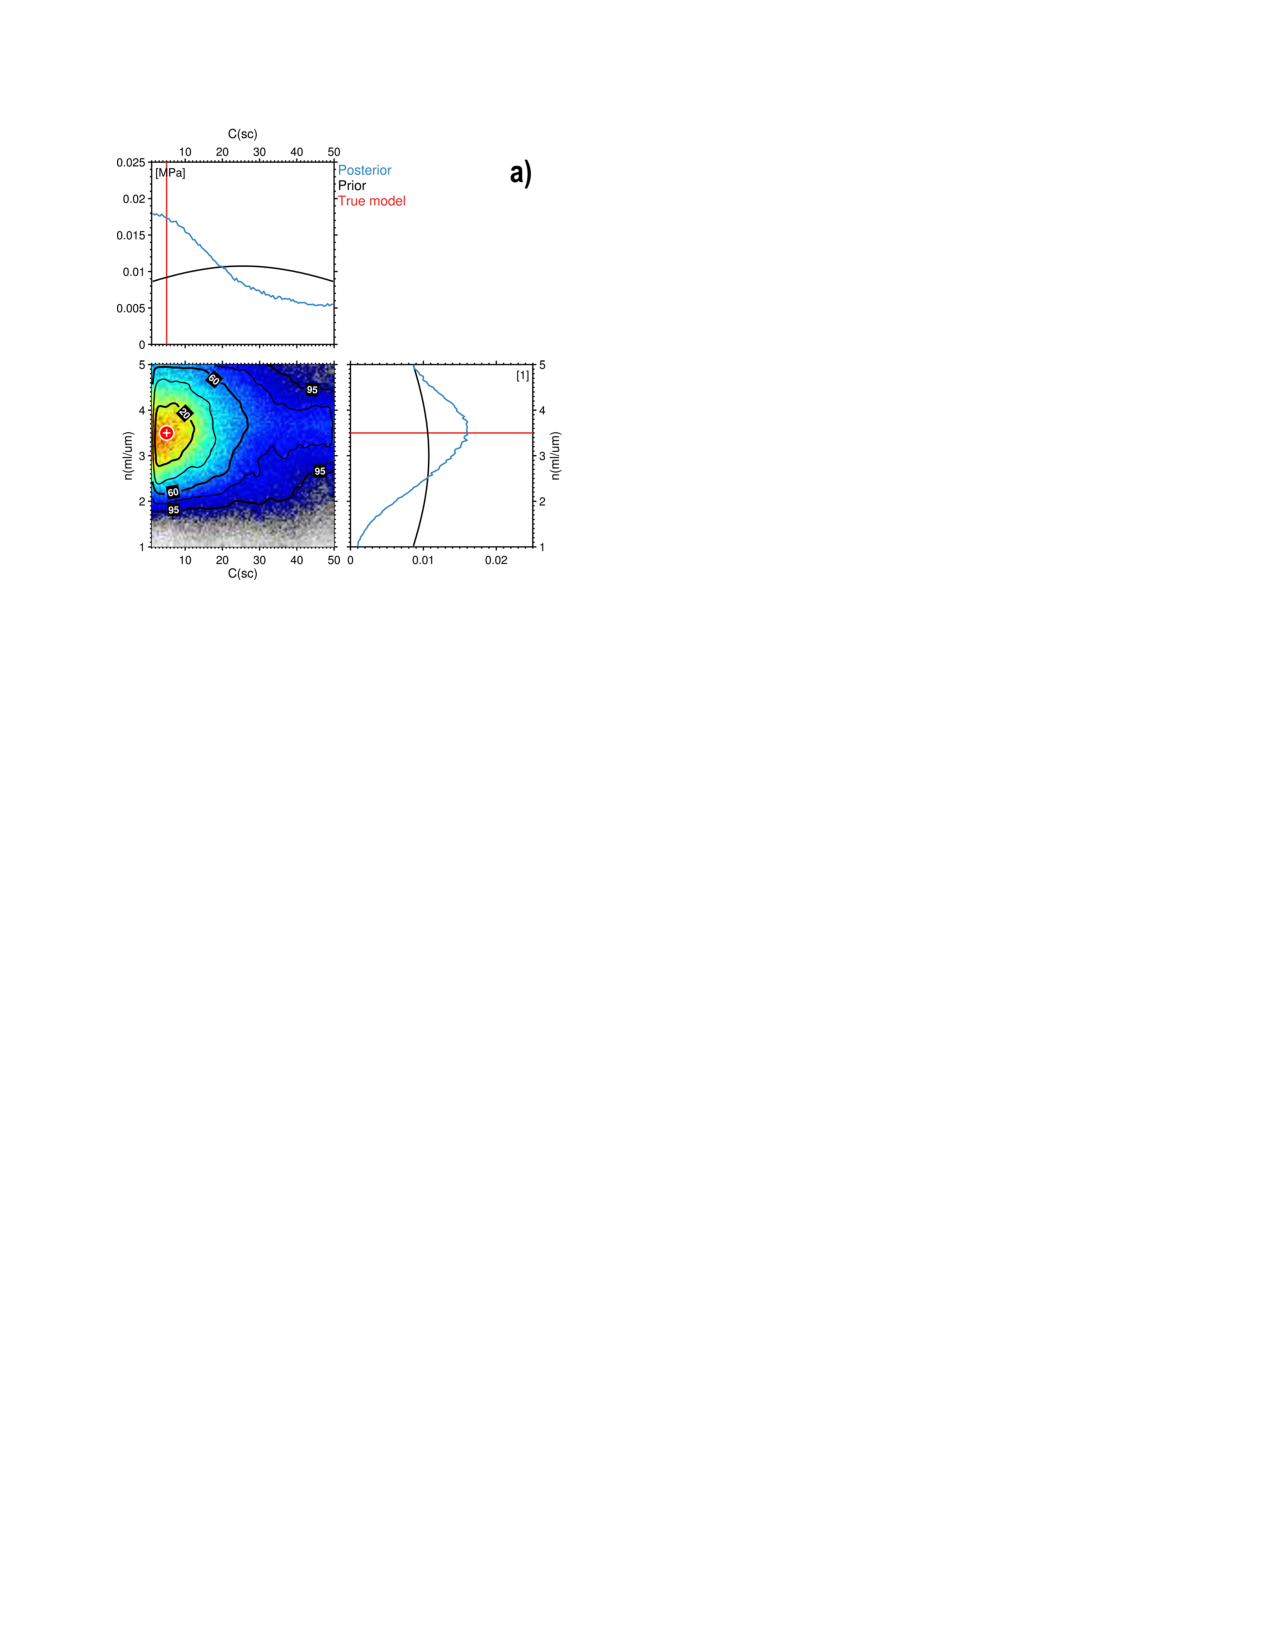
\includegraphics[height=0.8\textheight]{figures/Bayesian/BayesMCMCKaus}\\
\small Baumann and Kaus, 2015
\end{center}
\end{frame}
%
\begin{frame}{Strategy 2: Lots of Approximations}\Huge
\begin{center}
  \href{https://arxiv.org/pdf/1407.1517}{\parencite{buithanhgirolami2014}}
\end{center}

\bigskip

\begin{itemize}\LARGE
  \item[] Approx. posterior around the maximum (MAP) point
  \medskip
  \item[] Sample with MCMC
  \medskip
  \item[] Solve adjoint to get gradient of cost function
  \medskip
  \item[] Low-rank Hessian approximation
\end{itemize}
\end{frame}
%
\begin{frame}{Cross-Fade}\Huge
\begin{center}
  \href{https://academic.oup.com/gji/article/239/3/1629/7783283}{\parencite{minson2024}}
\end{center}

\bigskip

\begin{itemize}\LARGE
  \item[] Continuation method in distributions
  \medskip
  \item[] Does not require likelihood evaluations
  \medskip
  \item[] Calculates marginal likelihood for design optimization
\end{itemize}
\end{frame}
%
\begin{frame}[allowframebreaks]{References}
  \printbibliography
\end{frame}
%
\end{document}
